\subsection{Momentum Contrast (MoCo)}
\begin{frame}[allowframebreaks]{Momentum Contrast (MoCo)}
    \begin{figure}
        \centering
        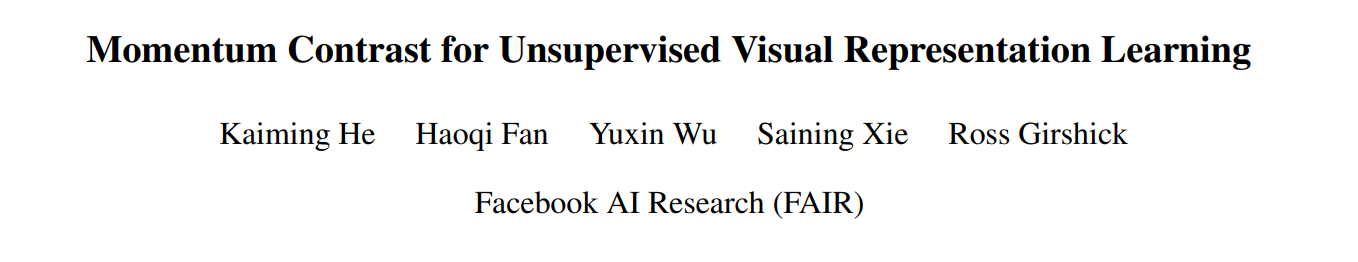
\includegraphics[width=1\linewidth,height=0.9\textheight,keepaspectratio]{images/ssl/slide_65_1_img.png}
    \end{figure}

    \framebreak

    \textbf{Momentum Contrast (MoCo)} is a self-supervised learning framework designed for visual representation learning. Its key components are:

    \vspace{0.5em}

    \textbf{Query \& Key Encoders}: Two neural networks, $f_q$ (query encoder) and $f_k$ (key encoder), are used. The key encoder $f_k$ is updated as an exponential moving average of the query encoder $f_q$:
        \[
            \theta_k \leftarrow m \theta_k + (1 - m) \theta_q
        \]
        where $\theta_k$ and $\theta_q$ are the parameters of $f_k$ and $f_q$, and $m$ is the momentum coefficient (e.g., $m=0.999$).
    
    \framebreak

    \begin{figure}
        \centering
        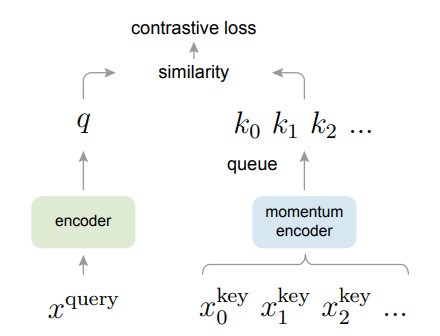
\includegraphics[width=1\linewidth,height=0.9\textheight,keepaspectratio]{images/ssl/slide_66_1_img.png}
    \end{figure}

    \framebreak

    \textbf{Dictionary Queue}: MoCo maintains a large queue (dictionary) of encoded keys from previous batches. This enables the use of a large and consistent set of negative samples for contrastive learning, which is crucial for effective representation learning.
    
    \vspace{0.5em}
    
    \textbf{Contrastive Loss}: The InfoNCE loss is used to train the encoders. For a given query $q$ and its positive key $k^+$, along with a set of negative keys $\{k_0, k_1, ..., k_N\}$ from the dictionary, the loss is:
        \[
            \mathcal{L}_{q} = -\log \frac{\exp(q \cdot k^+ / \tau)}{\exp(q \cdot k^+ / \tau) + \sum_{i=0}^{N} \exp(q \cdot k_i / \tau)}
        \]
        where $\tau$ is a temperature hyperparameter.

    \framebreak

    \begin{columns}
        \column{0.5\textwidth}
            \begin{figure}
                \centering
                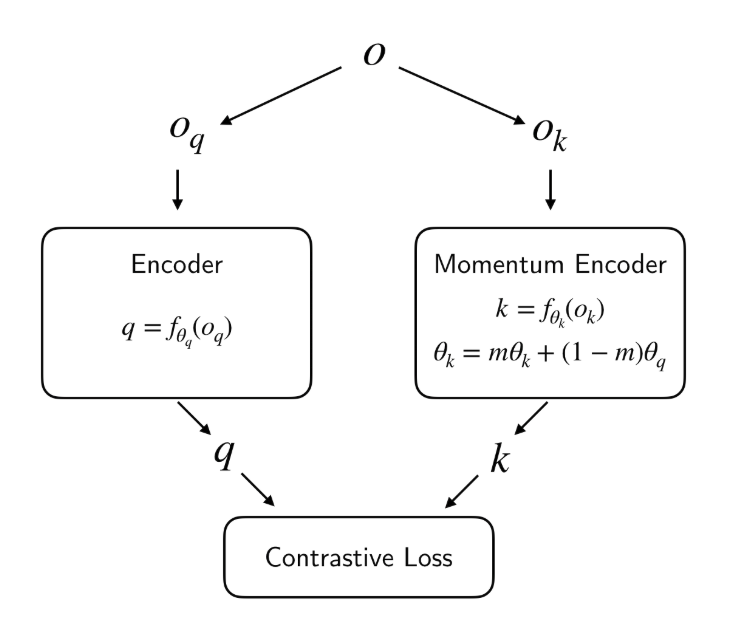
\includegraphics[width=1\linewidth,height=0.9\textheight,keepaspectratio]{images/ssl/slide_67_1_img.png}
            \end{figure}
        \column{0.5\textwidth}
            \begin{figure}
                \centering
                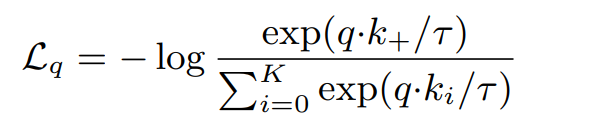
\includegraphics[width=1\linewidth,height=0.9\textheight,keepaspectratio]{images/ssl/slide_67_2_img.png}
            \end{figure}
    \end{columns}
    \framebreak

    \textbf{Key Steps in MoCo Training:}
    \begin{enumerate}
        \item For each image, generate two augmentations: one for the query encoder ($f_q$), one for the key encoder ($f_k$).
        \item Encode the query and key.
        \item Compute the InfoNCE loss using the current positive key and the dictionary of negative keys.
        \item Update $f_q$ via backpropagation; update $f_k$ via momentum.
        \item Enqueue the new key and dequeue the oldest key to maintain the dictionary size.
    \end{enumerate}

    \framebreak

    \begin{figure}
        \centering
        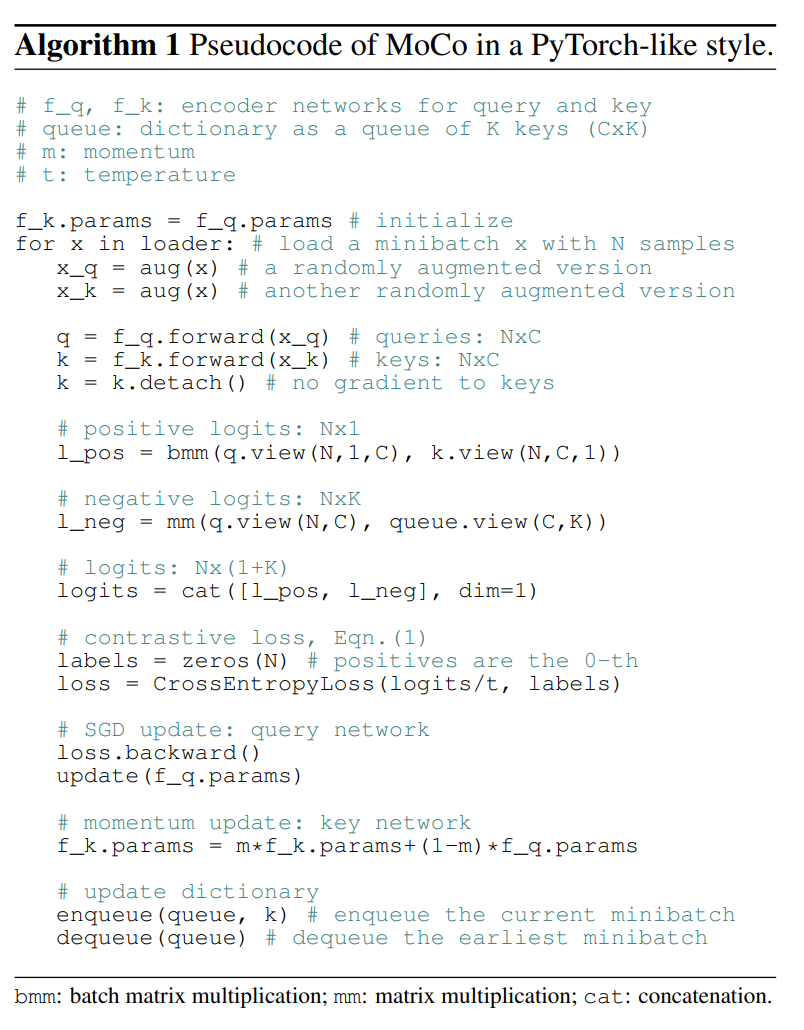
\includegraphics[width=1\linewidth,height=0.95\textheight,keepaspectratio]{images/ssl/slide_68_1_img.png}
    \end{figure}

    \framebreak

    \begin{figure}
        \centering
        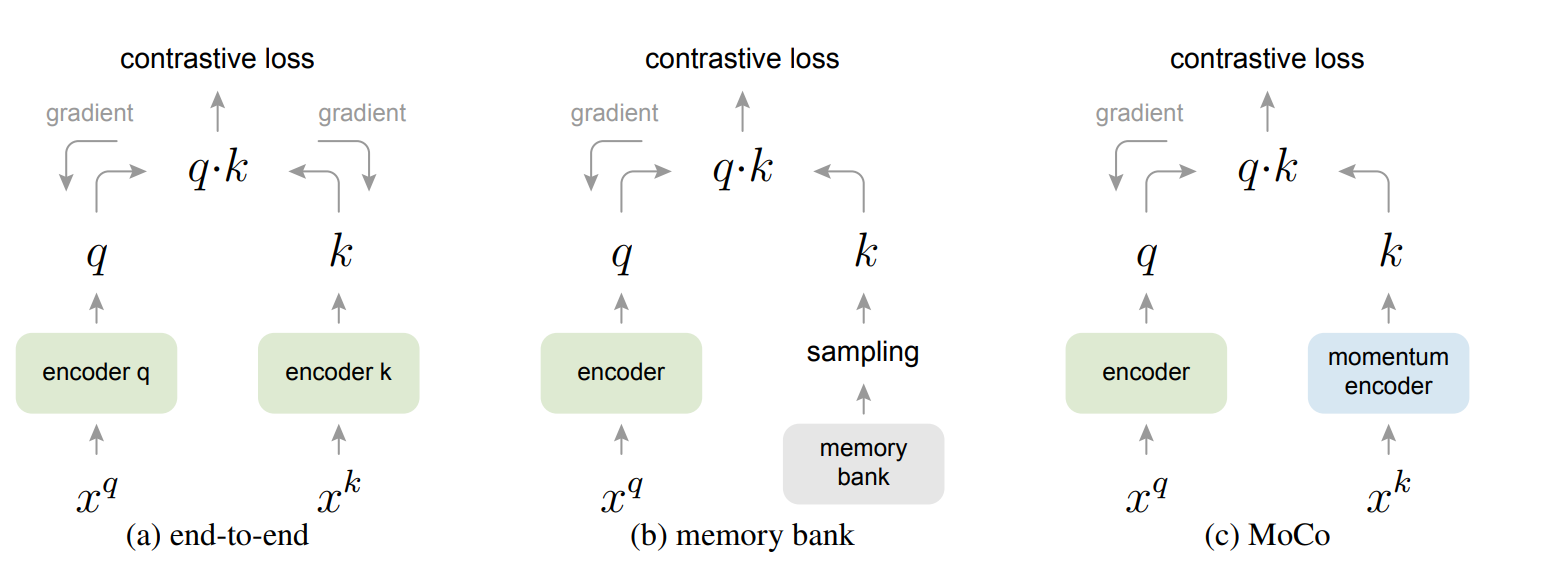
\includegraphics[width=1\linewidth,height=0.95\textheight,keepaspectratio]{images/ssl/slide_69_1_img.png}
    \end{figure}

    \framebreak

    \begin{figure}
        \centering
        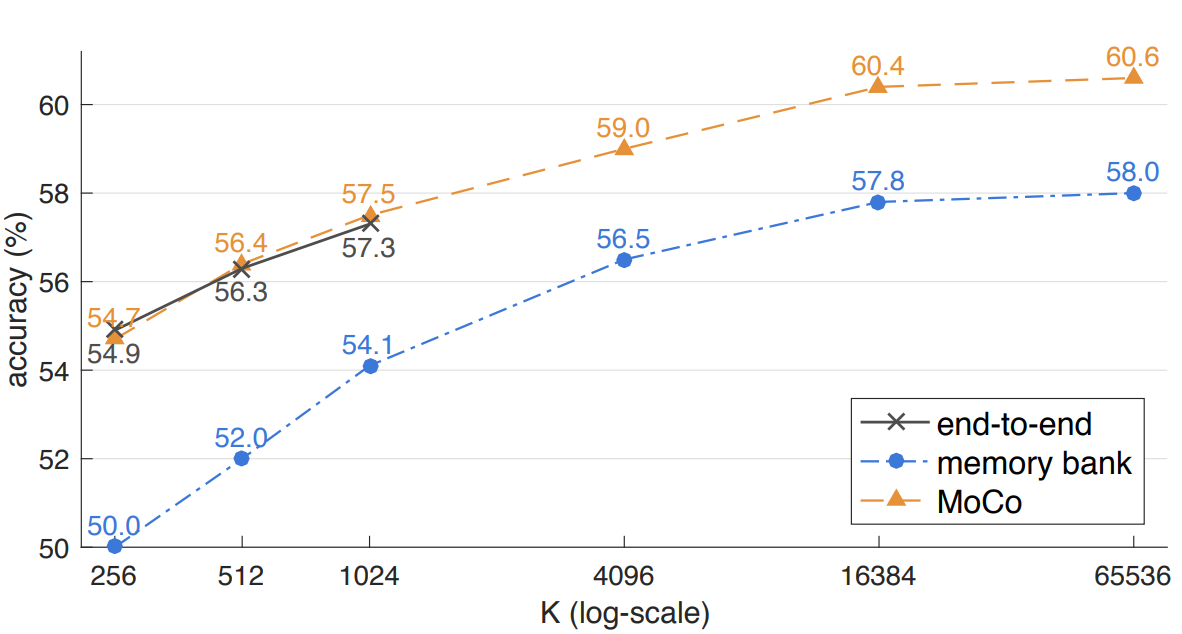
\includegraphics[width=1\linewidth,height=0.95\textheight,keepaspectratio]{images/ssl/slide_70_1_img.png}
    \end{figure}

    \framebreak

    \begin{figure}
        \centering
        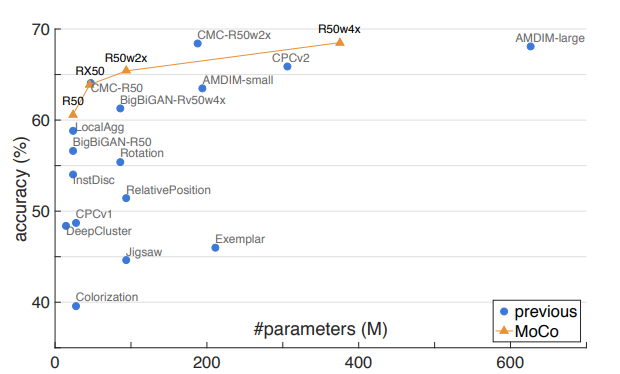
\includegraphics[width=1\linewidth,height=0.95\textheight,keepaspectratio]{images/ssl/slide_71_1_img.png}
    \end{figure}

    \framebreak

    \textbf{Key Advantages:}
    \begin{itemize}
        \item Enables large and consistent negative sets for contrastive learning.
        \item Momentum update stabilizes the key encoder, improving training.
        \item Scalable to large datasets and high-dimensional representations.
    \end{itemize}
\end{frame}